% 来源：OEBPS/Text/Section0001_split_007.xhtml#sigil_toc_id_52

\BookChapter{39}
\section[第39章\q 布恩·皮肯斯：努力致富，努力给予]{第39章\\ 布恩·皮肯斯：努力致富，努力给予}

\begin{figure}[htbp]
\centering
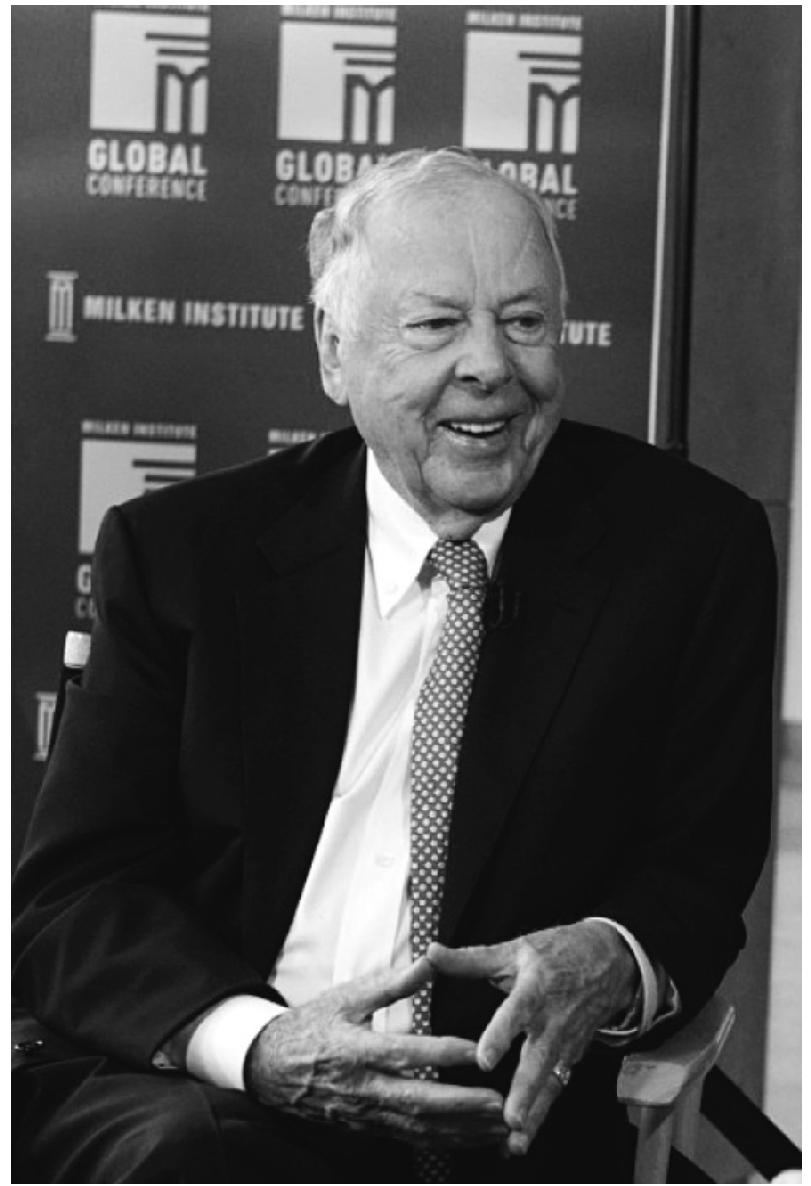
\includegraphics[width=0.40\linewidth,keepaspectratio]{image/布恩·皮肯斯肖像.jpg}
\caption*{布恩·皮肯斯}
\end{figure}

美国石油资本管理公司董事长兼首席执行官

布恩·皮肯斯，美国全国广播公司财经频道称其为“油神”，他总是能够超前自己所处的时代一大截。20世纪80年代早期，他是最早的一批公司袭击者，尽管他一直更喜欢“股东维权者”这个名号。布恩·皮肯斯早期重点关注的是股东价值最大化，那个时候几乎没有人听说过这种事，而现在股东价值最大化成了美国公司文化的一个标准。正如《财富》杂志所说的那样：“布恩·皮肯斯提出的曾经一度被认为是革命性的想法，现在大家一致认为这是理所当然的做法，而且是经济发展进步的关键所在。”

21世纪早期，皮肯斯成为一名对冲基金经理人，他年满70岁之后挣到了自己第一个10亿美元，通过投资能源类资产，他的职业生涯焕发了第二春。在接下来15年里，他把10亿美元变成了40亿美元，其中20亿美元后来又亏掉了，还有10亿美元捐了。

布恩·皮肯斯一直是个乐观主义者，最近第五次结婚。尽管已近90岁高龄，但他在社交媒体上有巨大的存在感，丝毫没有显露出慢下来的迹象。2013年布恩·皮肯斯未被列入《福布斯》美国400富豪排行榜，他发了一段非常有名的微博：“别担心。我还有9.5亿美元，我会做得很好。有意思的是，我捐了10亿美元，比我现在拥有的财富还要多。”我们俩交谈的时候，谈到个人财富缩水的事，布恩·皮肯斯说：“托尼，你是知道我的，我会再赚回来两个10亿美元，再过一两年就行。”

布恩·皮肯斯，1928年出生，正赶上美国经济大萧条，他起步的时候真是一无所有。12岁他就开始送报纸赚钱了，他最初送28种报纸，后来增长到156种报纸。他把这份少年时代的送报工作称为“通过并购实现增长”的入门课。1951年从俄克拉荷马州立大学毕业后，布恩·皮肯斯进入菲利普斯石油公司工作，1956年他自己创业，1964年他把自己的公司更名为梅萨石油公司，并逐步将其打造为得克萨斯州的一个能源王国。到1981年他的梅萨石油公司成为当时世界上最大的独立石油企业。布恩·皮肯斯在20世纪80年代的企业并购成为一个传奇，在此期间，海湾石油、菲利普斯石油、加利福尼亚州联合石油都一度成为他最著名的并购目标。

但是布恩·皮肯斯的运气（和财富）总是在变化。1996年他离开了梅萨石油公司，他创办的对冲基金公司的盈利螺旋式大幅度下滑，很多人都不把他当回事了——因为他很快就要亏损90\%的投资资本。但是布恩·皮肯斯上演了这个行业里的一个超级大反转，他把投资基金最后剩下的那300万美元又变成了好几十亿美元。

我们前面访谈的每位投资大师都主要关注两大资产类型——股票和债券，布恩·皮肯斯的英国石油资本公司的对冲基金却并非如此，他赌的是能源期货和衍生产品市场的走向。尽管本书致力于帮助人们取得财务独立，但布恩·皮肯斯说，美国过度依赖国外原油，这是最大的危险因素，对于美国整个国家安全来说是如此，对于我们经济上的幸福安宁也是如此。作为一个总是走在曲线之前的人，布恩·皮肯斯发起了一场改革运动，他要让美国这个国家摆脱对欧佩克（石油输出国组织）石油的依赖，他提出了皮肯斯计划，建议推行能源新政策。

我一直是布恩·皮肯斯的粉丝，从我长大能够记事起便一直如此，我现在很荣幸地能够称他为我的朋友。布恩·皮肯斯非常亲切和蔼，参加过我举办的很多场财富讲座活动，并发表演讲。下面的内容是我们最近谈话的节选，内容包括积累财富，保护美国能源的未来，还有他低微的出身。

\begin{BookQuote}
\textbf{罗宾斯：}我一开始想讲的第一件事是，你出生的那个不可思议的故事，你总是说，你是“世界上最幸运的家伙”，而且你这样说是很认真的。请给我们详细讲讲。
\end{BookQuote}

\begin{BookQuote}
\textbf{布恩·皮肯斯：}我的妈妈是1927年怀孕的，我是1928年5月出生的，在俄克拉荷马州乡下的一个小镇上。医生对我父亲说：“汤姆，现在你必须做出一个艰难的决定，要老婆还是要孩子，只能保住一个人的命。”我父亲说：“不可以，你肯定有办法，让母子两个人都能保住。”我们小镇上只有两个医生，幸运的是，给我妈妈接生的医生是个外科医生，他说：“好吧，汤姆，要做到你说的母子两个都保住，只能做剖宫产手术。我从来没有做过，但是我见过，我也读到过这方面的书，我可以展示给你看。”于是这位外科医生带着我父亲穿过房间，给他看一本书上有一页半讲剖宫产手术的内容。“汤姆，我要做的手术只写了这么一页半。”他说。我父亲读了一页半的内容，看着医生的眼睛说：“我想你肯定能做到。”他们两个人一起跪下来祈祷。后来他说服这个医生给我妈妈做了剖宫产手术，这才把我生出来了。
\end{BookQuote}

\begin{BookQuote}
\textbf{罗宾斯：}我的天哪！
\end{BookQuote}

\begin{BookQuote}
\textbf{布恩·皮肯斯：}又过了30年，他们那家医院才再一次做了一例剖宫产手术。
\end{BookQuote}

\begin{BookQuote}
\textbf{罗宾斯：}你父亲真是太有勇气了，关系到他深爱的妻儿两人的生命时，他也有勇气拒绝别人的建议，还有勇气说肯定有别的办法，他没有屈服。这件事肯定影响了你的人生，对不对？别人说不，你肯定不会轻易接受。
\end{BookQuote}

\begin{BookQuote}
\textbf{布恩·皮肯斯：}不会，我肯定不会。
\end{BookQuote}

\begin{BookQuote}
\textbf{罗宾斯：}你的父亲真是为你树立了一个榜样，有能力做出重大且困难的决策。你生下来了，你的妈妈也活得很好。多么美好的故事啊。我现在明白了，为什么你总是说你是“世界上最幸运的人”。
\end{BookQuote}

\begin{BookQuote}
\textbf{布恩·皮肯斯：}是的。
\end{BookQuote}

\begin{BookQuote}
\textbf{罗宾斯：}你说过，从小诚实的概念就深深影响了你。但是，不幸的是，在金融行业，很多人并不是把诚实当成做人做事的核心原则。
\end{BookQuote}

\begin{BookQuote}
\textbf{布恩·皮肯斯：}我十几岁时天天送报，有一天拿着报纸走在路上，无意间低头一看，忽然看见路边草丛上有什么东西，仔细一看，是个钱包。我拿起钱包，认出这是一个邻居怀特先生的，他就住在我送报的这条路上，他曾几次付钱给我，所以我记得这是他的钱包。于是我跑过去敲他家的门，见到他出来马上说：“怀特先生，我捡到了你的钱包。”他大叫一声：“哦，我的天哪！你可帮了我的大忙！谢谢你，我要好好感谢你。”怀特先生给了我1美元，我简直不敢相信，那个时候，1美元可是很大一笔钱，能买好多东西。
\end{BookQuote}

\begin{BookQuote}
\textbf{罗宾斯：}当然啦。
\end{BookQuote}

\begin{BookQuote}
\textbf{布恩·皮肯斯：}那是1940年，我才11岁。
\end{BookQuote}

\begin{BookQuote}
\textbf{罗宾斯：}噢。
\end{BookQuote}

\begin{BookQuote}
\textbf{布恩·皮肯斯：}于是我回到家里，我可高兴了，逐一告诉我的妈妈、婶婶、奶奶，我怎么碰巧捡到钱包还给怀特先生这件事，当然还要自豪地说，怀特先生给了我1美元。她们听了却都是摇头，我一看就知道她们不喜欢我讲的这件事。我说：“你们听明白了吗？怀特先生非常高兴，因为我捡到了他丢的钱包，赶紧把钱包还给他。”奶奶看着我说：“好孩子，你不应该因为诚实得到奖励。”于是我决定把这1美元还给怀特先生。
\end{BookQuote}

\begin{BookQuote}
\textbf{罗宾斯：}这种事肯定让人终生难忘！勇敢和诚实，这两个价值观确实塑造了你。我记得读到过你说的一句话，那时我还小，这句话让我很受启发。我总是非常着迷于这个问题，是什么东西让一个人成为一个领导者，而不是追随者。你说过你想按照自己的想法活出你自己的人生。我记得你让我小时候很受启发的那句话是：领导的秘密就是要决断。
\end{BookQuote}

\begin{BookQuote}
\textbf{布恩·皮肯斯：}1984年，我想收购海湾石油公司，我觉得这家公司的管理团队太弱了。我说：“这些人甚至都不敢扣动扳机。他们只是瞄准，再瞄准，却从来不会开火。”
\end{BookQuote}

\begin{BookQuote}
\textbf{罗宾斯：}你说得太形象了。那么你能够快速开火吗？
\end{BookQuote}

\begin{BookQuote}
\textbf{布恩·皮肯斯：}很多人是让人摆到领导位置上的，这让我气得发疯，因为这些人当了领导却不敢做决定。这些人不愿意自己做决定，他们希望别人来为他们做决定。我不一样，我能很快地做出决定，我觉得我做出的决定会很好，我会看到好的结果。
\end{BookQuote}

\begin{BookQuote}
\textbf{罗宾斯：}不错，结果才能证明理论是否正确。结果表明你的想法肯定是正确的。你成了拥有几十亿美元的大富翁，因为你对能源行业的理解更加准确，而且充分利用了这个优势做出正确的投资决策。
\end{BookQuote}

\begin{BookQuote}
\textbf{布恩·皮肯斯：}我21次预测油价，19次都预测准确。
\end{BookQuote}

\begin{BookQuote}
\textbf{罗宾斯：}21次预测对了19次，成功率太高了！
\end{BookQuote}

\begin{BookQuote}
\textbf{布恩·皮肯斯：}是的。我是在美国全国广播公司财经频道的节目上公开预测的。
\end{BookQuote}

\begin{BookQuote}
\textbf{罗宾斯：}这简直太不可思议了。你预测油价会达到每加仑4美元，是吧？当时是2011年，根本没有人想到油价会反弹到那么高。
\end{BookQuote}

\begin{BookQuote}
\textbf{布恩·皮肯斯：}我在你搞的讲座上演讲时公开说过，托尼，那是2011年在太阳谷，我冒着风险公开说，到7月4日美国独立日那个周末，我们会看到油价达到每桶120美元，结果确实如此。我记得我说，全球石油需求会上升到每天900亿桶，所以价格必须上涨，和这么高的需求水平相匹配。
\end{BookQuote}

\begin{BookQuote}
\textbf{罗宾斯：}我的很多白金合伙人，按照你的预测押注油价会涨，结果赚了很多钱。你让他们买入合成看涨期权，以充分利用那次油价上涨来赚钱。你的预测太准了，非常感谢你。那么，回顾你过去多年优异的历史业绩记录，有条主线，我在很多卓越的投资大师身上一次又一次地看到，那就是非常关注风险—收益不对称的机会。请问，你认为应该如何减少风险，或者如何确认冒这些风险和潜在收益相比是值得的？你在风险—收益不对称投资机会上的投资哲学是什么？
\end{BookQuote}

\begin{BookQuote}
\textbf{布恩·皮肯斯：}你如果读工商管理硕士，他们肯定会教你：减少你的下行风险，给你自己更大的上行收益，那么好的投资回报就会来了。但我从来不用这种方式做投资。
\end{BookQuote}

\begin{BookQuote}
\textbf{罗宾斯：}真的吗？
\end{BookQuote}

\begin{BookQuote}
\textbf{布恩·皮肯斯：}听我说，有些交易会比别的交易好得多。我想，我们在分析风险上做得很好，但是我不能具体告诉你，我究竟是怎么做出一个决策的。我知道，要是我击中了，我就能击出本垒打，也就是说我做对了，就会大赚特赚。同样的一件事，也许我会三振出局，就是说我也可能输得精光。我愿意承受大风险追求大回报。
\end{BookQuote}

\begin{BookQuote}
\textbf{罗宾斯：}好的，我明白了。那么，我来问问你这个问题：如果你的金融财富一分钱也不能传给你的孩子，只能传给孩子一套投资哲学，或者一套投资组合策略，那么会是什么？你会如何鼓励他们，好让他们能够长期投资之后拥有很大的财富？
\end{BookQuote}

\begin{BookQuote}
\textbf{布恩·皮肯斯：}我十分相信，如果你有一套好的工作规范，你要把它传给子孙后代。如果你有了良好的教育，再加上一套好的工作规范，你又愿意努力工作，我相信你肯定会实现自己的人生目标和财富目标。我觉得，我的那一套良好的工作规范，是在我的老家俄克拉荷马州那个小镇上学到的。我看到我的奶奶、妈妈、爸爸都非常努力地工作，我看到我周围的人都在努力地工作。我看到那些受过良好教育的人赚的钱更多。
\end{BookQuote}

\begin{BookQuote}
\textbf{罗宾斯：}听起来，你不是教给他们一个投资组合，你更想教给他们一套思维模式，一套工作规范。
\end{BookQuote}

\begin{BookQuote}
\textbf{布恩·皮肯斯：}是的，你说的对。
\end{BookQuote}

\begin{BookQuote}
\textbf{罗宾斯：}你赚到几十亿财富，又亏掉几十亿财富。钱对于你来说是什么？财富对于你来说又意味着什么？
\end{BookQuote}

\begin{BookQuote}
\textbf{布恩·皮肯斯：}我可以告诉你我过去什么时候觉得自己非常富有。
\end{BookQuote}

\begin{BookQuote}
\textbf{罗宾斯：}什么时候？
\end{BookQuote}

\begin{BookQuote}
\textbf{布恩·皮肯斯：}就是我有12只捕鸟猎狗的时候。
\end{BookQuote}

\begin{BookQuote}
\textbf{罗宾斯：}那时你多大年纪？
\end{BookQuote}

\begin{BookQuote}
\textbf{布恩·皮肯斯：}那时我50岁。
\end{BookQuote}

\begin{BookQuote}
\textbf{罗宾斯：}真的！
\end{BookQuote}

\begin{BookQuote}
\textbf{布恩·皮肯斯：}那一天我在打猎。我一直养捕鸟猎狗，我一直是个捕捉鹌鹑的猎手。我父亲是，我也是，但是我只是在后院养了一只捕鸟猎狗。后来我的捕鸟技术提高了，我就养了两只捕鸟猎狗。后来我养的捕鸟猎狗多到12只，我就建了一个狗屋。有一天我说：“你知道吗，我是一个大富豪了，我有12只捕鸟猎狗。”
\end{BookQuote}

\begin{BookQuote}
\textbf{罗宾斯：}你用你的财富给美国做了那么多有益的事。我知道，你是有史以来给大学捐赠最慷慨的人，你已经给你的母校俄克拉荷马州立大学捐赠了5亿多美元，这简直太让人吃惊了。
\end{BookQuote}

\begin{BookQuote}
\textbf{布恩·皮肯斯：}我的目标就是让俄克拉荷马州立大学变得更有竞争力，在运动上，在学术上，都更有竞争力。我非常荣幸能向我的母校捐赠。
\end{BookQuote}

\begin{BookQuote}
\textbf{罗宾斯：}你在2005年给俄克拉荷马州立大学运动队的捐赠，是美国大学生体育协会历史上最大的一笔捐赠，对吗？
\end{BookQuote}

\begin{BookQuote}
\textbf{布恩·皮肯斯：}是。
\end{BookQuote}

\begin{BookQuote}
\textbf{罗宾斯：}这太令人震惊了。我知道这只是你捐赠和给予的一部分而已，你的善举让我非常敬佩。让我们换个话题，谈谈能源独立这个大问题。你在石油行业发了大财。按理说，你应该最不可能是那个鼓吹美国能源独立的人，可是最近7年这却成了你的使命。请给我们讲讲你的皮肯斯计划。
\end{BookQuote}

\begin{BookQuote}
\textbf{布恩·皮肯斯：}我正想谈谈这个事。美国人是对石油上瘾了，这种油瘾威胁到了美国的经济、环境和国家安全。每过10年，这个问题就变得更加严重。1976年美国进口原油占比为24\%，现在美国进口原油占比接近70\%，而且比例还在不断提高。
\end{BookQuote}

\begin{BookQuote}
\textbf{罗宾斯：}所以你现在想把我们从那种石油进口依赖中解脱出来。
\end{BookQuote}

\begin{BookQuote}
\textbf{布恩·皮肯斯：}是的，我们把美国的国家安全放到了那些可能并不友好也并不稳定的外国政府手里。如果美国用的原油70\%都要依赖外国进口，那么在这个世事难料的世界上，美国就处在危险的境地。再过一个10年，美国进口原油的成本会达到10万亿美元，这会是人类历史上最大的财富转移。
\end{BookQuote}

\begin{BookQuote}
\textbf{罗宾斯：}这简直难以想象。你有什么解决方案吗？
\end{BookQuote}

\begin{BookQuote}
\textbf{布恩·皮肯斯：}我们应该搞能源升级，开发利用可再生能源，这能让美国获得巨大的好处，但是这并不能解决欧佩克问题。欧佩克是那些石油输出国搞的组织，实际上跟再生能源没有关系。风能和太阳能都是交通运输车辆可以使用的能源，天然气也可以派上大用场。全世界使用的原油总量，70\%是用在交通运输上的。我们要退出欧佩克实现能源独立自主，唯一的依靠就是美国自己的天然气，或者美国自己的原油。
\end{BookQuote}

\begin{BookQuote}
\textbf{罗宾斯：}那么我们应该怎么做？
\end{BookQuote}

\begin{BookQuote}
\textbf{布恩·皮肯斯：}美国每天要进口1200万桶原油，其中500万桶是从欧佩克国家进口的。我们需要在美国生产更多的天然气，才能摆脱从欧佩克进口这么多原油。我们有足够多的资源，完全能够做到这一点。托尼，我们现在就坐在天然气田上，我们座位下面的天然气储量足够美国使用100年。我们的天然气储量相当于4万亿桶原油，这是沙特阿拉伯原油储量的3倍。如果美国不能充分利用自己如此巨大的天然气资源，我们就会和最愚蠢的螃蟹爬到城里的下场一样。
\end{BookQuote}

\begin{BookQuote}
\textbf{罗宾斯：}这太让我震惊了。
\end{BookQuote}

\begin{BookQuote}
\textbf{布恩·皮肯斯：}天然气现在非常便宜。100美元买1桶原油，按照油气当量，相当于16美元买到1立方米天然气的热量，可是我们从来没有见过天然气价格达到过1立方米16美元。不管是运输还是发电，现在任何人使用能源都应该优先考虑更加便宜的天然气。
\end{BookQuote}

\begin{BookQuote}
\textbf{罗宾斯：}我知道你花了自己很多时间、精力、金钱，宣传你的这个皮肯斯计划。你把你的计划传播给美国公众，出钱在全国范围宣传，在媒体上大打广告，这么大的投入有效果吗？
\end{BookQuote}

\begin{BookQuote}
\textbf{布恩·皮肯斯：}2008年，我在华盛顿发起了皮肯斯计划，我用自己的钱在这个计划上投入了1亿美元。我觉得，在争取美国能源独立自主这件事上，我能做的事情我都做了，这是美国的大事，我们要给美国搞一个能源计划。
\end{BookQuote}

\begin{BookQuote}
\textbf{罗宾斯：}在本书里我谈了很多资产配置。可以说，你把所有资产都配置在能源行业上了。你人生中大多数时候都是这样重仓能源行业，对吗？
\end{BookQuote}

\begin{BookQuote}
\textbf{布恩·皮肯斯：}你说的对，但是在能源行业里有很多不同的板块。我们的投资横跨整个能源领域，但是没有超出能源行业这个大板块。
\end{BookQuote}

\begin{BookQuote}
\textbf{罗宾斯：}这是你个人独特版本的资产配置。如果你是一个普通的个人投资者，今天要做投资，比如你现在手里只有5万美元可以投资，你会把这5万美元投到哪里？
\end{BookQuote}

\begin{BookQuote}
\textbf{布恩·皮肯斯：}我会投资到能源行业的下游，在这里你会看到一些炼油公司等。我这辈子大部分时间都花在能源行业的上游，主要是做勘探和开采。但是现在天然气比石油便宜了。天然气行业非常有吸引力，这是一个值得投资者关注的领域。总体而言，我觉得石油和天然气行业，有着非常光明的未来，这是因为科技的发展进步。我们在科技上的进步，简直令人难以置信。从自然能源的角度来看，美国现在看起来要比10年前做得好多了。10年前我可不是这样想的，那时我可不像现在这样对美国未来的能源状况充满信心。
\end{BookQuote}

\begin{BookQuote}
\textbf{罗宾斯：}请问，是什么在驱动你一路奋斗？
\end{BookQuote}

\begin{BookQuote}
\textbf{布恩·皮肯斯：}托尼，你知道，在现在这个时间点上，驱动我的动力是我喜欢赚钱。我也喜欢捐钱，相比之下我更喜欢赚钱，但二者非常接近。我坚信，我能幸运地来到世界上，有一个原因是要成功，要赚大钱，要慷慨大方地花大钱。
\end{BookQuote}

\begin{BookQuote}
\textbf{罗宾斯：}慷慨大方地花大钱？
\end{BookQuote}

\begin{BookQuote}
\textbf{布恩：}慷慨大方地捐大钱。我有个人生目标，就是要在生前捐出10亿美元。你知道巴菲特和比尔·盖茨发起的给予誓言行动吗？就是自愿捐出一半的个人财富。他们打电话给我，让我参加。我说：“你看一下1983年以来的《财富》杂志，你们为什么不加入我搞的俱乐部？我在这个俱乐部里说了，我要捐出90\%的个人财富，比你们号召捐出的50\%还要多出40\%。”
\end{BookQuote}

\begin{BookQuote}
\textbf{罗宾斯：}你的捐赠比例真是太高了。
\end{BookQuote}

\begin{BookQuote}
\textbf{布恩·皮肯斯：}每天我都去办公室上班，我天天早上盼望着去办公室上班。我这辈子一直都是这样过来的。所以我的工作对于我来说就是一切，但是你可能会说“不，我的家庭对于我来说才是一切，你不能那样说，工作并不是一切”。应该说，工作和家庭都充满乐趣。我和家人在一起的时候，很有乐趣，我工作的时候，也很有乐趣。结果并不完美，但是已经够好了，它能让你觉得，第二天你会来个本垒打，大赢一把。也许后来没有大赢一把，但我仍然认为每天我都有机会大赢一把。
\end{BookQuote}

\begin{BookQuote}
\textbf{罗宾斯：}你启发了我，就像你启发了世界上很多人一样。我受到你的激情感染和全力以赴的启发。布恩·皮肯斯，现在你80多岁了，取得了这么多非凡的成就之后，你还在持续进步，持续成长，持续给予。
\end{BookQuote}

\begin{BookQuote}
\textbf{布恩·皮肯斯：}谢谢你，托尼，你也一直是个非常成功的人，帮助了很多人，也许你帮助的人比我还多。
\end{BookQuote}

\begin{BookQuote}
\textbf{罗宾斯：}噢，我也不知道帮过多少人。
\end{BookQuote}

\begin{BookQuote}
\textbf{布恩·皮肯斯：}但是我们俩都是人生赢家，因为我们俩真的在持续给予。
\end{BookQuote}

\begin{BookQuote}
\textbf{罗宾斯：}这一点我同意。我非常敬重你，我的好朋友。谢谢你！
\end{BookQuote}
